
%    \documentclass[journal,a4paper]{IEEEtran}
\documentclass[10pt,twocolumn,twoside]{IEEEtran}

%% 88mm column width
% 18.2cms full page

   % \documentclass[draftcls,onecolumn]{IEEEtran} 
   % \topmargin       -6.0mm
   %  \oddsidemargin      0mm
   %  \evensidemargin     0mm
   %  \textheight     223.5mm
   % \textwidth      170.0mm




% If IEEEtran.cls has not been installed into the LaTeX system files,
% manually specify the path to it like:
% \documentclass[journal]{../sty/IEEEtran}





% Some very useful LaTeX packages include:
% (uncomment the ones you want to load)


% *** MISC UTILITY PACKAGES ***
%
%\usepackage{ifpdf}
% Heiko Oberdiek's ifpdf.sty is very useful if you need conditional
% compilation based on whether the output is pdf or dvi.
% usage:
% \ifpdf
%   % pdf code
% \else
%   % dvi code
% \fi
% The latest version of ifpdf.sty can be obtained from:
% http://www.ctan.org/tex-archive/macros/latex/contrib/oberdiek/
% Also, note that IEEEtran.cls V1.7 and later provides a builtin
% \ifCLASSINFOpdf conditional that works the same way.
% When switching from latex to pdflatex and vice-versa, the compiler may
% have to be run twice to clear warning/error messages.






% *** CITATION PACKAGES ***
%
\usepackage{cite}


% *** GRAPHICS RELATED PACKAGES ***
%
\ifCLASSINFOpdf
   \usepackage[pdftex]{graphicx}
  % declare the path(s) where your graphic files are
  % \graphicspath{{../pdf/}{../jpeg/}}
  % and their extensions so you won't have to specify these with
  % every instance of \includegraphics
  % \DeclareGraphicsExtensions{.pdf,.jpeg,.png}
\else
  % or other class option (dvipsone, dvipdf, if not using dvips). graphicx
  % will default to the driver specified in the system graphics.cfg if no
  % driver is specified.
  % \usepackage[dvips]{graphicx}
  % declare the path(s) where your graphic files are
  % \graphicspath{{../eps/}}
  % and their extensions so you won't have to specify these with
  % every instance of \includegraphics
  % \DeclareGraphicsExtensions{.eps}
\fi


% *** MATH PACKAGES ***
%
\usepackage[cmex10]{amsmath}
\interdisplaylinepenalty=2500

\usepackage{amssymb}




% *** ALIGNMENT PACKAGES ***
%
\usepackage{array}



%\usepackage{mdwmath}
%\usepackage{mdwtab}
% Also highly recommended is Mark Wooding's extremely powerful MDW tools,
% especially mdwmath.sty and mdwtab.sty which are used to format equations
% and tables, respectively. The MDWtools set is already installed on most
% LaTeX systems. The lastest version and documentation is available at:
% http://www.ctan.org/tex-archive/macros/latex/contrib/mdwtools/



% *** SUBFIGURE PACKAGES ***
% \usepackage[tight,footnotesize]{subfigure}

 \ifCLASSOPTIONcompsoc
  \usepackage[tight,normalsize,sf,SF]{subfigure}
\else
  \usepackage[tight,footnotesize]{subfigure}
\fi


%\usepackage[caption=false]{caption}
%\usepackage[font=footnotesize]{subfig}
% subfig.sty, also written by Steven Douglas Cochran, is the modern


% *** FLOAT PACKAGES ***
%
%\usepackage{fixltx2e}
% fixltx2e, the successor to the earlier fix2col.sty, was written by
% Frank Mittelbach and David Carlisle. This package corrects a few problems
% in the LaTeX2e kernel, the most notable of which is that in current
% LaTeX2e releases, the ordering of single and double column floats is not
% guaranteed to be preserved. Thus, an unpatched LaTeX2e can allow a
% single column figure to be placed prior to an earlier double column
% figure. The latest version and documentation can be found at:
% http://www.ctan.org/tex-archive/macros/latex/base/



\usepackage{stfloats}
% stfloats.sty was written by Sigitas Tolusis. This package gives LaTeX2e
% the ability to do double column floats at the bottom of the page as well
% as the top. (e.g., "\begin{figure*}[!b]" is not normally possible in
% LaTeX2e). It also provides a command:
%\fnbelowfloat
% to enable the placement of footnotes below bottom floats (the standard
% LaTeX2e kernel puts them above bottom floats). This is an invasive package
% which rewrites many portions of the LaTeX2e float routines. It may not work
% with other packages that modify the LaTeX2e float routines. The latest
% version and documentation can be obtained at:
% http://www.ctan.org/tex-archive/macros/latex/contrib/sttools/
% Documentation is contained in the stfloats.sty comments as well as in the
% presfull.pdf file. Do not use the stfloats baselinefloat ability as IEEE
% does not allow \baselineskip to stretch. Authors submitting work to the
% IEEE should note that IEEE rarely uses double column equations and
% that authors should try to avoid such use. Do not be tempted to use the
% cuted.sty or midfloat.sty packages (also by Sigitas Tolusis) as IEEE does
% not format its papers in such ways.


%\ifCLASSOPTIONcaptionsoff
%  \usepackage[nomarkers]{endfloat}
% \let\MYoriglatexcaption\caption
% \renewcommand{\caption}[2][\relax]{\MYoriglatexcaption[#2]{#2}}
%\fi
% endfloat.sty was written by James Darrell McCauley and Jeff Goldberg.
% This package may be useful when used in conjunction with IEEEtran.cls'
% captionsoff option. Some IEEE journals/societies require that submissions
% have lists of figures/tables at the end of the paper and that
% figures/tables without any captions are placed on a page by themselves at
% the end of the document. If needed, the draftcls IEEEtran class option or
% \CLASSINPUTbaselinestretch interface can be used to increase the line
% spacing as well. Be sure and use the nomarkers option of endfloat to
% prevent endfloat from "marking" where the figures would have been placed
% in the text. The two hack lines of code above are a slight modification of
% that suggested by in the endfloat docs (section 8.3.1) to ensure that
% the full captions always appear in the list of figures/tables - even if
% the user used the short optional argument of \caption[]{}.
% IEEE papers do not typically make use of \caption[]'s optional argument,
% so this should not be an issue. A similar trick can be used to disable
% captions of packages such as subfig.sty that lack options to turn off
% the subcaptions:
% For subfig.sty:
% \let\MYorigsubfloat\subfloat
% \renewcommand{\subfloat}[2][\relax]{\MYorigsubfloat[]{#2}}
% For subfigure.sty:
% \let\MYorigsubfigure\subfigure
% \renewcommand{\subfigure}[2][\relax]{\MYorigsubfigure[]{#2}}
% However, the above trick will not work if both optional arguments of
% the \subfloat/subfig command are used. Furthermore, there needs to be a
% description of each subfigure *somewhere* and endfloat does not add
% subfigure captions to its list of figures. Thus, the best approach is to
% avoid the use of subfigure captions (many IEEE journals avoid them anyway)
% and instead reference/explain all the subfigures within the main caption.
% The latest version of endfloat.sty and its documentation can obtained at:
% http://www.ctan.org/tex-archive/macros/latex/contrib/endfloat/
%
% The IEEEtran \ifCLASSOPTIONcaptionsoff conditional can also be used
% later in the document, say, to conditionally put the References on a 
% page by themselves. 
\usepackage{float}
 \usepackage{hyperref}
\hypersetup{colorlinks,linkcolor=black,filecolor=black,urlcolor=black,citecolor=black}

\usepackage{color}
\newcommand{\dean}[1]{\textsf{\emph{\textbf{\textcolor{red}{#1}}}}} 
\newcommand{\parham}[1]{\textsf{\emph{\textbf{\textcolor{blue}{#1}}}}}


% *** PDF, URL AND HYPERLINK PACKAGES ***
%
%\usepackage{url}
% url.sty was written by Donald Arseneau. It provides better support for
% handling and breaking URLs. url.sty is already installed on most LaTeX
% systems. The latest version can be obtained at:
% http://www.ctan.org/tex-archive/macros/latex/contrib/misc/
% Read the url.sty source comments for usage information. Basically,
% \url{my_url_here}.





% *** Do not adjust lengths that control margins, column widths, etc. ***
% *** Do not use packages that alter fonts (such as pslatex).         ***
% There should be no need to do such things with IEEEtran.cls V1.6 and later.
% (Unless specifically asked to do so by the journal or conference you plan
% to submit to, of course. )


% correct bad hyphenation here
\hyphenation{op-tical net-works semi-conduc-tor}


\begin{document}
%
% paper title
% can use linebreaks \\ within to get better formatting as desired
\title{Non-Parametric Estimation of Integro-Difference Equation Based Spatio-Temporal Systems}
%
%
% author names and IEEE memberships
% note positions of commas and nonbreaking spaces ( ~ ) LaTeX will not break
% a structure at a ~ so this keeps an author's name from being broken across
% two lines.
% use \thanks{} to gain access to the first footnote area
% a separate \thanks must be used for each paragraph as LaTeX2e's \thanks
% was not built to handle multiple paragraphs
%

\author{Parham Aram, Dean R. Freestone, 
        Michael Dewar, David B. Grayden, Visakan Kadirkamanathan~\IEEEmembership{Member,~IEEE} and Kenneth Scerri  % <-this % stops a space
\thanks{P. Aram and V. Kadirkamanathan are with the Department of Automatic Control and Systems Engineering, University of Sheffield, Sheffield, S1 3JD, U.K. (e-mail:  p.aram@sheffield.ac.uk; visakan@sheffield.ac.uk).}% <-this % stops a space
\thanks{D. R. Freestone and D. B. Grayden are with the Department of Electrical and Electronic Engineering, The University of Melbourne,
Parkville, VIC, Australia (e-mail:deanrf@unimelb.edu.au; grayden@unimelb.edu.au).}
\thanks{M. Dewar is with bit.ly, New York City, USA (e-mail:md@bit.ly)}  
\thanks{K. Scerri is with the Department of Systems and Control Engineering, University of Malta, Msida, MSD, Malta (e-mail:kenneth.scerri@um.edu.mt).}\thanks{P. Aram and D. R. Freestone contributed equally to this work.}} 




%\thanks{Manuscript received April 19, 2005; revised January 11, 2007.}}

% note the % following the last \IEEEmembership and also \thanks - 
% these prevent an unwanted space from occurring between the last author name
% and the end of the author line. i.e., if you had this:
% 
% \author{....lastname \thanks{...} \thanks{...} }
%                     ^------------^------------^----Do not want these spaces!
%
% a space would be appended to the last name and could cause every name on that
% line to be shifted left slightly. This is one of those "LaTeX things". For
% instance, "\textbf{A} \textbf{B}" will typeset as "A B" not "AB". To get
% "AB" then you have to do: "\textbf{A}\textbf{B}"
% \thanks is no different in this regard, so shield the last } of each \thanks
% that ends a line with a % and do not let a space in before the next \thanks.
% Spaces after \IEEEmembership other than the last one are OK (and needed) as
% you are supposed to have spaces between the names. For what it is worth,
% this is a minor point as most people would not even notice if the said evil
% space somehow managed to creep in.



% The paper headers
\markboth{IEEE TRANSACTIONS ON SIGNAL PROCESSING}%
{Aram \MakeLowercase{\textit{et al.}}: A Non-Parametric Method for Integro-Difference Equation-Based Spatio-Temporal Systems}
% The only time the second header will appear is for the odd numbered pages
% after the title page when using the twoside option.
% 
% *** Note that you probably will NOT want to include the author's ***
% *** name in the headers of peer review papers.                   ***
% You can use \ifCLASSOPTIONpeerreview for conditional compilation here if
% you desire.




% If you want to put a publisher's ID mark on the page you can do it like
% this:
%\IEEEpubid{0000--0000/00\$00.00~\copyright~2007 IEEE}
% Remember, if you use this you must call \IEEEpubidadjcol in the second
% column for its text to clear the IEEEpubid mark.



% use for special paper notices
%\IEEEspecialpapernotice{(Invited Paper)}




% make the title area
\maketitle


\begin{abstract}
%\boldmath
The integro-difference equation (IDE) is an increasingly popular mathematical model of spatio-temporal processes, such as brain dynamics, weather systems, disease spread and others. Here we develop a non-parametric framework for fusing the IDE with data. The method is based on the average (over time) spatial correlations of data to estimate the spatial mixing kernel, disturbance and the noise parameters. Synthetic examples are given to demonstrate the performance of the estimation algorithm. % The proposed method can be also applied prior to the expectation maximization (EM) algorithm to provide better and efficient state and parameter estimation.
\end{abstract}
% IEEEtran.cls defaults to using nonbold math in the Abstract.
% This preserves the distinction between vectors and scalars. However,
% if the journal you are submitting to favors bold math in the abstract,
% then you can use LaTeX's standard command \boldmath at the very start
% of the abstract to achieve this. Many IEEE journals frown on math
% in the abstract anyway.

% Note that keywords are not normally used for peerreview papers.
\begin{IEEEkeywords}
dynamic spatio-temporal modelling, integro-difference equation (IDE).
\end{IEEEkeywords}






% For peer review papers, you can put extra information on the cover
% page as needed:
% \ifCLASSOPTIONpeerreview
% \begin{center} \bfseries MEDICS Category: 3-BBND \end{center}
% \fi
%
% For peerreview papers, this IEEEtran command inserts a page break and
% creates the second title. It will be ignored for other modes.
\IEEEpeerreviewmaketitle



\section{Introduction}
\IEEEPARstart{T}{he} ability to describe the spatio-temporal dynamics of systems has a profound effect on the manner in which we deal with the natural and man-made world. Complex spatio-temporal behavior is found in many different systems, such as aquatic ecosystems \cite{Schofield2002}, meteorological forecasting \cite{Xu2005}, air pollution \cite{Romanowicz2006}, soil temperature  \cite{Bond-Lamberty2005}, chemical processes \cite{Deng2005}, disease spread \cite{Kuo2009} and real estate markets \cite{Pace2000,Sun2005}. Spatio-temporal mathematical modeling aims to represent dynamic system behavior simultaneously, by diffusion or spread through space and evolution through time \cite{Cressie2011}. This paper introduces a new method for fusing the integro-difference equation (IDE) spatio-temporal model with sampled data. %For example, understanding the development of structures from dividing cells in the early embryo by modeling the chemical processes~\cite{Maini1997}. Another example is modeling functional resonance imaging (fMRI) to spatially localize neural activity in the brain \cite{Woolrich2004}. 
% Another example is modeling conflicts to capture important geographical features of the war scenarios \cite{Zammit-Mangion2012}. 
%\cite{Schofield2002,Xu2005,Romanowicz2006,Bond-Lamberty2005,Deng2005,Kuo2009,Sun2005}.  %WEINAND1972  

Techniques for modeling spatio-temporal systems are generating growing interest, both in the applied and theoretical literature. This interest is perhaps driven by increasing computational power and an ever increasing fidelity of spatio-temporal measurements of various systems. Computational models to describe spatio-temporal processes of particular interest in the wider literature include the cellular automata (CA) \cite{Wolfram1994}, coupled map lattices (CMLs) \cite{Billings2002}, lattice dynamical wavelet neural network (LDWNN) \cite{Wei2009}, spatially correlated time series \cite{Pfeifer1980,Glasbey2008,Dewar2007}, and the IDE. These models have all been used in a system identification context. The extent of the spatial interactions in these models is determined by a spatially discrete neighborhood structure. This paper deals in particular with the IDE-based spatio-temporal models. 

The focus on the IDE-based models in this work is due their relevance in describing the dynamics of the electrical fields of the brain~\cite{Deco2008,Schiff2008,Freestone2011}. IDE models are also relevant for describing other systems, where diffusion processes govern the dynamics, such as in population ecology and spread of organisms \cite{Kot1992,Kot1996}. The key feature of IDE models is that they combine discrete temporal dynamics with a continuous spatial representation. The dynamics of this model are governed by a spatial mixing kernel, which defines the mapping between the consecutive spatial fields (see~\figurename{\ref{fig:IDEConcept}}). The IDE model can be applied to data sampled both regularly and irregularly in space due to the continuous representation of each spatial field.  

\begin{figure}[ht]
	\centering
		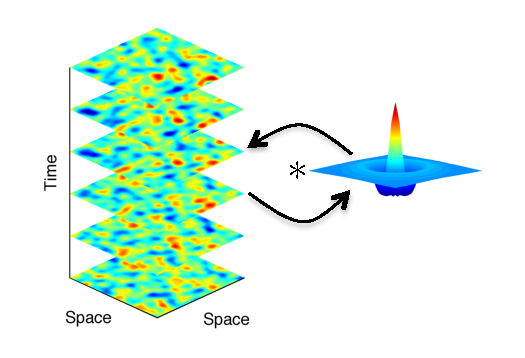
\includegraphics[scale=1]{./Graph/FieldsAndKernel_Arrows.pdf}
	\caption{Spatio-temporal IDE model. The evolution of the spatial field is governed by the spatial mixing kernel. In the case of homogeneous kernel the spatial field evolves through a convolution integral. At each time instant, the spatial field is subject to disturbance (see equation \eqref{eq:ConvolutionIntegral}). }
	\label{fig:IDEConcept}
\end{figure}

Estimating the spatial mixing kernel and the underlying spatial field is of particular interest and can be achieved by using conventional state-space modeling \cite{Dewar2009,Scerri2009} or in a hierarchical Bayesian framework \cite{Wikle1999,Xu2005,Wikle2011}. Wikle et al. \cite{Wikle2004} addressed the estimation problem by describing the IDE in a state-space formulation by decomposing the kernel and the field using a set of spectral basis functions. An alternative approach for the decomposition of the IDE and estimation of the spatial mixing kernel, using the expectation maximization (EM) algorithm, was introduced by Dewar et al. \cite{Dewar2009}. The key development of this work was a framework where the state and parameter space dimensions were independent of the number of observation locations. % In this work a framework based on expectation maximization (EM)  algorithm \cite{Dempster1977,Gibsona2005}  was used to estimate both the field and the kernel from the observed data.  
The problem of an efficient decomposition of the spatial mixing kernel and the field was addressed in Scerri et al. \cite{Scerri2009}, by incorporating the estimated support of the spatial mixing kernel and the spatial bandwidth of the system from observations. 
% (the temporal average of spatial cross-correlation of the consecutive observations) 
 % (the temporal average of the spatial spectrum of the observed fields) 
% Therefore, increasing the resolution at which the system is observed does not necessarily increase the complexity of the system identification problem.
 % A similar approach is adopted by \cite{Scerri2009} which developed a model selection procedure by considering various spatial scales at which to represent the system.
A heuristic approximate estimate of the kernel support obtained by the temporal average of spatial cross-correlation of the consecutive observations.  

Here we further develop the work of Scerri et al. \cite{Scerri2009}, by establishing an efficient method for estimating the spatial mixing kernel, the field disturbance characteristics, and the observation noise variance. The estimates are given by closed-form equations, based on the average (over time) spatial auto-correlation and cross-correlation of the observed field. This eliminates the computational load imposed by the methods in Dewar et al. and Scerri et al. \cite{Dewar2009,Scerri2009}. Furthermore, we relax assumptions in the previous work where they assumed that disturbance and noise characteristics were known to the estimator. Although the proposed method does not infer the underlying field from observed data, the results from the new methods can be used as a prerequisite for the EM-based algorithms (see \cite{Dewar2009,Xu2007}), providing better and efficient state (spatial field) and parameter estimations (spatial mixing kernel). 

The rest of this paper is set out as follows. In Section 2 the stochastic IDE model is briefly reviewed. Section 3 describes the derivation of the estimation framework and provides necessary formulations to construct such an estimator using the observed field. In Section 4, synthetic examples are given to demonstrate the estimation performance. Finally, conclusions are drawn in Section 5. All symbols used in the subsequent sections are given in Table.~\ref{table:Notation}. 
\begin {table}[t]
\begin{center}
	{\tiny\begin{tabular}{llll}
	\hline \hline
	& Symbol & Quantity & Units\\ 
	\hline 
	& Domain&& \\
	& $\Omega$ &Spatial domain& n.a. \\ 
	& $\mathbb{Z}^{+}$ &Non-negative integers& n.a. \\ 
	& $\mathbf{r}$ &Spatial location& arbitrary unit\\ 
	& $t$ &Time & s \\  
 	% & $\boldsymbol{\nu}$ &Spatial frequency& arbitrary unit\\  
	& $\mathbf I$ & Identity matrix & n.a. \\ 
 	%& $\ast$ & Convolution operator & n.a. \\ 
 	%& $\star$ & Correlation operator & n.a. \\ 
  % & $\mathcal{F}\{\cdot\}$ &Fourier transform& n.a. \\  
  %  & $\mathcal{F}^{-1}\{\cdot\}$ &Inverse Fourier transform& n.a. \\  
  % & $\mathbf{E}[\cdot]$ &Expectation operator& n.a. \\  

	& Model&& \\
	& $\mathbf{y}_t$ & Observation & Arbitrary unit \\
	& $z_t(\mathbf{r})$ & Spatial field & Arbitrary unit \\ 
	& $f_t(\mathbf{r})$ & Sigmoidal function & spike~s$^{-1}$ \\ 
	& $g_t(\mathbf{r})$ & Weighted sigmoidal function & spike~s$^{-1}$ \\
 	& $e_t(\mathbf{r})$ & Field disturbance, with covariance function $\gamma(\mathbf{r}-\mathbf{r'})$  & spike~s$^{-1}$ \\
 	& $\varepsilon_t$ & Observation noise, with covariance matrix $\Sigma_{\varepsilon}$  & mV \\  
 	& $m(\mathbf{r}-\mathbf{r'})$ & Observation kernel& n.a. \\  
 	& $k(\mathbf{r}-\mathbf{r'})$ & Spatial mixing kernel& n.a. \\ 
	&$\psi_i$&kernel basis function&n.a.\\
	&$\theta_i$ &Connectivity kernel parameters&mVspike$^{-1}$ \\ 
	& $\boldsymbol\mu_i$ &Kernel centers& mm \\  
	& $\sigma_{i}$ &kernel width parameters&mm \\ 
 	% & $\delta(t)$ &Dirac-delta function& n.a. \\  
 	%  	& $\delta(\boldsymbol\tau)$ &Kronecker delta& n.a. \\  
	& Estimation&& \\
 	& $\boldsymbol\tau$ &Spatial shift& Arbitrary unit \\
  & $\hat{f}(\cdot)$ &Linearized sigmoidal function around the threshold& spike~s$^{-1}$ \\  
  & $R_{y_{t+1}y_t}(\boldsymbol{\tau}) $ &The spatial cross-correlation between consecutive observations& arbitrary unit \\  
  & $R_{y_{t+1}y_{t+1}}(\boldsymbol{\tau})$ & The spatial auto-correlation at time $t+1$& arbitrary unit \\    
 	\hline \hline
	\end{tabular}}
 \caption {Notation. 	The symbols, description of the quantity, and the SI units where relevant.} 
 \label{table:Notation}
 \end{center}
 \end {table}

\section{Stochastic IDE Model}
The form of the spatially homogeneous IDE that is used for the examples in this paper is the Amari style neural field model. This was chosen since it generalizes to more simple IDE models that are commonly used in the literature with particular parameter settings. The stochastic Amari neural field model (see \cite{Freestone2011} for more details) is given by the equation  
\begin{equation}
 z_{t+1}\left(\mathbf{r}\right)=\xi z_t(\mathbf{r})+T_s\int_{\Omega}k\left(\mathbf{r}-\mathbf{r}'\right)f(z_{t}\left(\mathbf{r}'\right))d\mathbf{r}'+e_{t}\left(\mathbf{r}\right),
\label{eq:ConvolutionIntegral}
\end{equation}
where $t\in \mathbb{Z}^{+} $ denotes discrete time, $T_s$ is the sampling time step and $\mathbf{r} \in \Omega \subset \mathbb{R}^{n}$ are spatial locations in $n \in \left\lbrace 1,2,3 \right\rbrace $-dimensional physical space. The parameter $\xi$ is a decay term that is used to model synaptic dynamics in neural field models. In more simple forms of the IDE decay parameter is set to zero to model pure diffusion processes. The continuous spatial field at time $t$ and at location $\mathbf r$ is denoted $z_t\left(\mathbf r\right)$. The spatial dynamics are defined by the homogeneous time invariant spatial mixing kernel, $k\left(\mathbf{r}\right)$, which maps the field through time (which may be transformed or scaled by the activation function $f(\cdot)$) via the convolution defined in \eqref{eq:ConvolutionIntegral}. In the case of the neural field model example that we will employ in this paper, $f(\cdot)$ takes the form of a sigmoidal function or a linearized sigmoid function in the forward model and is always approximated as a linearized function in the estimator. These functions are given by
\begin{align}
	\label{ActivationFunction} f\left( z_t\left( \mathbf{r}'\right) \right) =& \frac{1}{1 + \exp \left( \varsigma \left( z_0 - z_t\left(\mathbf{r}'\right) \right) \right)} \\
	\hat{f}(z_t\left(\mathbf{r}\right)) &=\frac{2 + \varsigma(z_t\left(\mathbf{r}\right) - z_0)}{4}, 
\end{align}
where $\hat{f}(z_t\left(\mathbf{r}\right))$ is linearized about the threshold $z_0$. The parameter $\varsigma$ defines the slope of the activation function. The disturbance $e_{t}(\mathbf{r})$ is a zero-mean normally distributed noise process, spatially colored but temporally independent, with covariance \cite{Rasmussen2005}
\begin{equation}
cov\left(e_{t}\left(\mathbf{r}\right),e_{t+t'}\left(\mathbf{r'}\right)\right)=\sigma_d^2\delta(t-t')\gamma(\mathbf{r}-\mathbf{r'}),
\label{eq:FieldDisturbance}
\end{equation}
where $\sigma_d$ is temporal disturbance, $\delta(t)$ is the Dirac-delta function and $\gamma(\mathbf{r}-\mathbf{r'})$ is a spatially homogeneous covariance function. The mapping between the spatial field and the observations, denoted by $\mathbf{y}_t(\mathbf{r}_n)$, is modeled using the observation function that incorporates sensors with a spatial extent
\begin{equation}\label{eq:ObservationEquation}
	y_t(\mathbf{r}_n) = \int_{\Omega} { m\left(\mathbf{r}-\mathbf{r}'\right) z_t\left(\mathbf{r}'\right) \, d\mathbf{r}'} + \varepsilon_t(\mathbf{r}_n), 
\end{equation}
where $m\left(\mathbf{r}\right)$ is the observation kernel and $\varepsilon_t(\mathbf{r}_n) \sim \mathcal{N}\left(0,\boldsymbol{\Sigma}_{\varepsilon}\right)$ denotes a multivariate normal distribution with mean zero and the covariance matrix $\boldsymbol{\Sigma}_{\varepsilon} = \sigma_{\varepsilon}^2\mathbf{I}$, where $\mathbf{I}$ is the identity matrix.
% defined in this work by the Gaussian

\section{Estimation Method}\label{sec:EstimationMethod}
For the derivation of the spatial properties estimator of the field equations we assume \dean{the forward model} has a nonlinear sigmoidal activation function. This is common in computational modeling of mesoscopic brain dynamics to describe the relationship between the mean membrane potential and mean firing rate of a given population of neurons \cite{Freeman1975}. The results obtained using the sigmoidal function can be easily modified to account for other linear forms of the IDE that are used in other models of electrophysiological data, and furthermore, modeling in other areas such as population ecology and weather nowcasting. This is described in a later section in more details. 

To proceed we will switch to a more compact notation to define convolution and correlation operators. The spatial convolution shall be denoted as
\begin{equation}
	\int_\Omega a(\mathbf{r}-\mathbf{r}')b(\mathbf{r}')d\mathbf{r}' = (a\ast b)(\mathbf{r}),
\end{equation}
and the spatial cross-correlation shall be denoted as 
\begin{equation}
	\int_\Omega a(\mathbf{r})b(\mathbf{r}+\boldsymbol{\tau})d\mathbf{r} = (a\star b)(\boldsymbol{\tau}),
\end{equation} 
where $\boldsymbol{\tau}$ is the spatial shift.

\subsection{Estimation of spatial mixing kernel} 
The shape of the spatial mixing kernel can be inferred by studying the spatial cross-correlation between consecutive observations under the assumption that the sensors are not spatially band-limiting (i.e. have a wider bandwidth than the connectivity kernel and disturbance covariance), and the spatial mixing kernel is homogeneous.  To begin the derivation we define the spatial cross-correlation between consecutive observations (in time) as  
% The spatial relationship between consecutive observations is governed by the shape of the mixing kernel. 
% The deterministic component of the spatial mapping of the current field is due to the convolution of the kernel with the previous field. Therefore, the spatial cross-correlation between consecutive observations is used to estimate the kernel's support and shape.
\begin{equation}
	R_{y_{t+1}y_t}(\boldsymbol{\tau}) = \left(y_{t+1}\star y_t\right)\left(\boldsymbol{\tau}\right).
\end{equation}
The goal of the derivation is to make the necessary substitutions and simplifications to get an expression of the cross-correlation as a function of the mixing kernel. In the next step we substitute \eqref{eq:ObservationEquation} for $y_{t+1}(\mathbf{r})$ and expand to give
\begin{equation}
	R_{y_{t+1}y_t}\left(\boldsymbol{\tau}\right) = \left(\left(m \ast z_{t+1}\right)\star y_t\right)\left(\boldsymbol{\tau}\right) + \left(\varepsilon_{t+1} \star y_t\right)\left(\boldsymbol{\tau}\right).
\end{equation}
Next we substitute \eqref{eq:ConvolutionIntegral} for $z_{t+1}(\mathbf{r})$ giving 
\begin{align}
	R_{y_{t+1}y_t}&(\boldsymbol{\tau}) = (\left(m \ast \left(\xi z_t +  T_s g_t + e_t\right)\right) \star y_t)(\boldsymbol{\tau}) \nonumber\\
	&= \xi\left(\left(m \ast z_t\right) \star y_t \right)(\boldsymbol{\tau})+ T_s \left(\left(m\ast g_t\right)\star y_t \right)(\boldsymbol{\tau}) \nonumber\\
	&\quad+ \left(\left(m\ast e_t\right)\star y_t \right)(\boldsymbol{\tau})+ (\varepsilon_{t+1} \star y_t)(\boldsymbol{\tau}),
\end{align}
where
\begin{equation}\label{eq:averagefiringrate}
	g_t(\mathbf r)=\int_{\Omega}k\left(\mathbf{r}-\mathbf{r}'\right)f(z_{t}\left(\mathbf{r}'\right))d\mathbf{r}'.
\end{equation}
Now we take the expectation over time, so that the observation noise and process disturbance terms have minimal effect on the result, giving 
\begin{align}\label{eq:ExpectationToCancelNoise}
	\mathbf{E}[R_{y_{t+1}y_t}(\boldsymbol{\tau})] &= \mathbf{E}[\xi\left(\left(m \ast z_t\right) \star y_t \right)(\boldsymbol{\tau})] \nonumber \\
	 &\quad+ T_s \mathbf{E}[\left(\left(m\ast g_t\right)\star y_t \right)(\boldsymbol{\tau})],
\end{align}
since the disturbance and measurement noise are assumed to be independent of the observations and temporally white. Now by substituting $y_t - \varepsilon_t$ for $m\ast z_t$ from \eqref{eq:ObservationEquation} the first term of above equation can be written as
\begin{align}
	\mathbf{E}[\xi&\left(\left(m \ast z_t \right) \star y_t \right)(\boldsymbol{\tau})] = \mathbf{E}\left[\xi\left(\left(y_t-\varepsilon_t\right) \star y_t \right)(\boldsymbol{\tau})\right] \nonumber \\
	&= \xi \mathbf{E}\left[ (y_t \star y_t)(\boldsymbol{\tau}) - \left(\varepsilon_t\star y_t \right)(\boldsymbol{\tau})\right] \nonumber \\
	&= \xi\mathbf{E}[ R_{y_ty_t}(\boldsymbol{\tau})  - \left(\varepsilon_t \star (m\ast z_t + \varepsilon_t)\right) (\boldsymbol{\tau})] \nonumber \\
	&=\xi\mathbf{E}[ R_{y_ty_t}(\boldsymbol{\tau}) -\left(\varepsilon_t\star (m\ast z_t)\right)(\boldsymbol{\tau}) - (\varepsilon_t\star\varepsilon_t)(\boldsymbol{\tau})] \nonumber\\ 
	&= \xi\left(\mathbf{E}[ R_{y_ty_t}(\boldsymbol{\tau})] - \sigma_{\varepsilon}^2 \delta(\boldsymbol{\tau})\right), \label{eq:FirstTermReduced}
\end{align}
where $\delta(\boldsymbol\tau)$ denotes Kronecker delta. Next we simplify second term in equation \eqref{eq:ExpectationToCancelNoise} to get an expression involving the spatial mixing kernel. By substituting equation \eqref{eq:averagefiringrate} for $g_t$ we can write
\begin{equation}\label{eq:before_linearization}
	T_s((m \ast g_t) \star y_t)(\boldsymbol\tau) = T_s((k \ast m\ast f(z_t)) \star y_t)(\boldsymbol\tau).
\end{equation}   
The remainder of the derivation is focused on isolating the spatial mixing kernel on the left hand side. In order to achieve this, we need to assume a linear activation function. The linearized activation function is introduced to equation~\eqref{eq:before_linearization} to get
\begin{align}	
	T_s((m \ast g_t) \star y_t)(\boldsymbol\tau) \approx \frac{T_s}{4}((k\ast (c_1 + \varsigma m \ast z_t)) \star y_t)(\boldsymbol\tau), 
\end{align}
where
\begin{equation}
	c_1 = m\ast (2 - \varsigma z_0),
\end{equation}
is a constant. Now by substituting $y_t - \varepsilon_t$ in for $m\ast v_t$ we can write
\begin{align}
	T_s((m \ast g_t) \star y_t)(\boldsymbol\tau) &\approx \frac{T_s}{4}((k\ast (c_1 + \varsigma (y_t - \varepsilon_t))) \star y_t) (\boldsymbol\tau).
\end{align}
To isolate the kernel, the order of the convolution and cross-correlation is reversed by recognizing that a property $(a \ast b)(\boldsymbol\tau) \star c(\boldsymbol\tau) = a(-\boldsymbol\tau)\ast(b \star c)(\boldsymbol\tau)$ (see Appendix~\ref{ap:CorrelationAnalysis}). Therefore,
\begin{align}
	T_s((m \ast g_t) \star y_t)(\boldsymbol\tau) &\approx \frac{T_s}{4} k(-\boldsymbol\tau) \ast ((c_1 + \varsigma (y_t - \varepsilon_t)) \star y_t)(\boldsymbol\tau) \nonumber\\
	= \frac{T_s}{4}k(-\boldsymbol\tau) & \ast (( c_t + \varsigma (y_t - \varepsilon_t)) \star y_t) (\boldsymbol\tau),
\end{align}
where
\begin{equation}
	c_t = (c_1\star y_t)(\boldsymbol\tau).
\end{equation}  
Now using the identity established to get equation~\eqref{eq:FirstTermReduced}, we have
\begin{align}\label{eq:second_term_reduced}
	T_s\mathbf{E}&\left[((m \ast g_t) \star y_t)(\boldsymbol\tau)\right] \approx \nonumber \\
	&\frac{T_s}{4} k(-\boldsymbol\tau) \ast (\mathbf{E}\left[c_t(\boldsymbol\tau)\right] + \varsigma (\mathbf{E}\left[R_{y_ty_t}(\boldsymbol\tau)\right] - \sigma_{\varepsilon}^2 \delta(\boldsymbol\tau)))
\end{align}
Substituting back equation~\eqref{eq:second_term_reduced} into equation~\eqref{eq:ExpectationToCancelNoise} we get
\begin{align}\label{eq:SimplifiedXcorr}
	\mathbf{E}&[R_{y_{t+1}y_t}(\boldsymbol{\tau})] \approx \xi\left(\mathbf{E}[ R_{y_ty_t}(\boldsymbol{\tau})] - \sigma_{\varepsilon}^2 \delta(\boldsymbol{\tau})\right) \nonumber \\
	&\quad+ \frac{T_s}{4} k(-\boldsymbol\tau) \ast (\mathbf{E}\left[c_t(\boldsymbol\tau)\right] + \varsigma (\mathbf{E}\left[R_{y_ty_t}(\boldsymbol\tau)\right] - \sigma_{\varepsilon}^2 \delta(\boldsymbol\tau))).
\end{align}
Rearranging equation~\eqref{eq:SimplifiedXcorr} we get
\begin{align} \label{eq:Tobesolvedforthekernel}
	k(-\boldsymbol\tau) & \ast (\mathbf{E}\left[c_t(\boldsymbol\tau)\right] + \varsigma (\mathbf{E}\left[R_{y_ty_t}(\boldsymbol\tau)\right] - \sigma_{\varepsilon}^2 \delta(\boldsymbol\tau))) \approx  \nonumber \\
	& \frac{4}{T_s}(\mathbf{E}[R_{y_{t+1}y_t}(\boldsymbol{\tau})] - \xi\left(\mathbf{E}[ R_{y_ty_t}(\boldsymbol{\tau})] - \sigma_{\varepsilon}^2 \delta(\boldsymbol{\tau})\right)).
\end{align}
The solution of the above equation for the mixing kernel is a deconvolution. Using the convolution theorem equation~\eqref{eq:Tobesolvedforthekernel} can be solved for the kernel in the frequency domain giving,
\begin{align}
	\mathcal{F}&\{k(-\boldsymbol\tau)\} \approx  \nonumber \\
	&= \frac{4}{T_s} \frac{\mathcal{F}\{\mathbf{E}[R_{y_{t+1}y_t}(\boldsymbol{\tau})]\} - \xi\left(\mathcal{F}\{\mathbf{E}[ R_{y_ty_t}(\boldsymbol{\tau})]\} - \sigma_{\varepsilon}^2 \right)} {\mathcal{F}\{\mathbf{E}\left[c_t(\boldsymbol\tau)\right]\} + \varsigma (\mathcal{F}\{\mathbf{E}\left[R_{y_ty_t}(\boldsymbol\tau)\right]\} - \sigma_{\varepsilon}^2 )}.  \label{eq:Fourier_TF_of_Kernel}
\end{align} 
Finally an expression for the kernel is obtained by taking the inverse Fourier transform giving 
\begin{align}\label{eq:EM-Fourier_TF_of_Kernel}   
	k&(\boldsymbol\tau) = \nonumber \\
	&\frac{4}{T_s}\mathcal{F}^{-1}\overline{\left\{ \frac{\mathcal{F}\{\mathbf{E}[R_{y_{t+1}y_t}(\boldsymbol{\tau})]\} - \xi\left(\mathcal{F}\{\mathbf{E}[ R_{y_ty_t}(\boldsymbol{\tau})]\} - \sigma_{\varepsilon}^2 \right)}{\mathcal{F}\{\mathbf{E}\left[c_t(\boldsymbol\tau)\right]\} + \varsigma (\mathcal{F}\{\mathbf{E}\left[R_{y_ty_t}(\boldsymbol\tau)\right]\} - \sigma_{\varepsilon}^2 )} \right\}},
\end{align}
 where over-bar denotes the complex conjugate operator. As the mixing kernel is a real function, the complex conjugate operator essentially reflects the kernel through the origin in the spatial domain \cite{Bracewell2000}. In the case of isotropic kernel, the complex conjugate operator can be dropped. 

In the case where $f(z_t(\mathbf{r}))=z_t(\mathbf{r})$, it can be shown that the solution given by \eqref{eq:EM-Fourier_TF_of_Kernel} is simplified to  
\begin{equation}\label{eq:SimplifiedKernelSolution}
	k(\boldsymbol\tau) = \frac{1}{T_s }\mathcal{F}^{-1}\overline{\left\{\frac{\mathcal{F}\{\mathbf{E}[R_{y_{t+1}y_t}(\boldsymbol{\tau})]\}}{\mathcal{F}\{(\mathbf{E}\left[R_{y_ty_t}(\boldsymbol\tau)\right]\} - \sigma_{\varepsilon}^2 }-\xi\right\}}.
\end{equation}
This is in fact a spacial case for the general solution given by equation~\eqref{eq:EM-Fourier_TF_of_Kernel} with $\varsigma=4$ and $z_0=0.5$ in equation~\eqref{eq:linearizeSigmoid}. From equation~\eqref{eq:SimplifiedKernelSolution} we see that an error in our guess for $\xi$ will result in a shift of the estimated kernel amplitude and an error in the initial guess of the observation noise variance will result in a distortion in the shape of the kernel. However, if the signal-to-noise ratio is high such a distortion becomes insignificant. The equation \eqref{eq:SimplifiedKernelSolution} can be further simplified by setting the decay parameter, $\xi=0$ to model diffusion processes. Setting the sampling time $T_s=1$ solves the linear IDE studied in \cite{Dewar2009, Scerri2009}.  
% An incorrect estimate of $c_t$ will result in a DC scaling (\parham{or shift?}) in the kernel estimate

By the Wiener-Khintchine theorem (WKT) the denominator of \eqref{eq:SimplifiedKernelSolution} is equivalent to the power spectral density (PSD) which is non-negative and a real quantity \cite{Ricker2003}. The WKT allows to establish the bounds on the initial guess of $\sigma_{\varepsilon}^2$
% The WKT states that the power spectral density of the wide sense stationary process is the Fourier transform of its auto-correlation function .
\begin{equation}\label{eq:BoundOnObsVariance}   
  \min\mathcal{F}\{(\mathbf{E}\left[R_{y_ty_t}(\boldsymbol\tau)\right]\}\ge\sigma_{\varepsilon}^2\ge0. 
\end{equation}
In practice, we have found that 
\begin{equation}
	\min\mathcal{F}\{(\mathbf{E}\left[R_{y_ty_t}(\boldsymbol\tau)\right]\}\approx\sigma_{\varepsilon}^2,
\end{equation}
although we have no formal proof.

\subsection{Estimation of disturbance covariance function}
The field disturbance at each spatial location and at a given time is correlated with other spatial locations through the disturbance covariance
function. This suggests that the auto-correlation of the observed field at each time instant may provide useful information about the field disturbance characteristics.
The observation auto-correlation at time $t+1$ can be expressed as
\begin{equation}\label{eq:EM-ObservationEquationAutocorrelation}
	R_{y_{t+1}y_{t+1}}(\boldsymbol{\tau})=(y_{t+1} \star y_{t+1})(\boldsymbol\tau).
\end{equation}
 After substituting for $y_{t+1}$ from \eqref{eq:ObservationEquation} and using equation~\eqref{eq:ConvolutionIntegral}   for $z_{t+1}$,  equation~\eqref{eq:EM-ObservationEquationAutocorrelation} is expanded to give 
\begin{align}\label{eq:EM-expanded_auto_corr}  
	R_{y_{t+1}y_{t+1}} & (\boldsymbol{\tau}) = \\ \nonumber 
	\left( \left(\xi( m\ast z_{t}) \right.\right.&+\left.\left. T_s(m\ast g_{t}) + ( m \ast e_{t})+\varepsilon_{t+1} \right) \star y_{t+1} \right) (\boldsymbol{\tau}).
\end{align}
Now we expand to get
\begin{align}\label{eq:expanded_auto_corr}
	R_{y_{t+1}y_{t+1}}&(\boldsymbol{\tau}) = \xi((m \ast z_{t}) \star y_{t+1})(\boldsymbol{\tau})+T_s((m\ast g_{t})\star y_{t+1})(\boldsymbol{\tau}) \nonumber \\
	&\quad+((m\ast e_{t})\star  y_{t+1})(\boldsymbol{\tau})+(\varepsilon_{t+1} \star y_{t+1})(\boldsymbol{\tau}).
\end{align}
By using similar arguments that were used in the derivation for the mixing kernel, the auto-correlation can be simplified by recognizing that
\begin{align}\label{eq:EM-Autoterm1} 
  \mathbf{E}[\xi((m\ast z_{t})\star y_{t+1})(\boldsymbol{\tau})]&=\xi \mathbf{E}[ R_{y_ty_{t+1}}(\boldsymbol{\tau})],
\end{align}
\begin{align}\label{eq:EM-Autoterm2}
 (\varepsilon_{t+1}\star y_{t+1})(\boldsymbol\tau)&=\sigma_{\varepsilon}^2\delta(\boldsymbol{\tau}),
\end{align} 
and
\begin{align}\label{eq:EM-Autoterm3} 
	T_s\mathbf{E}[((m\ast g_t) &\star y_{t+1})(\boldsymbol\tau)] \nonumber \\ 
	&\approx \frac{T_s}{4}\mathbf{E}[((m \ast k \ast (2 + \varsigma z_t - \varsigma z_0))\star y_{t+1})(\boldsymbol\tau)] \nonumber \\
	&= \frac{T_s}{4} w(-\boldsymbol\tau) \ast (\mathbf{E}\left[c_t\right] + \varsigma \mathbf{E}\left[R_{y_ty_{t+1}}(\boldsymbol\tau)\right] ).
\end{align}
Substituting \eqref{eq:EM-Autoterm1}, \eqref{eq:EM-Autoterm2} and ~\eqref{eq:EM-Autoterm3} back into \eqref{eq:expanded_auto_corr} and taking the expectation over time  gives
\begin{align}\label{eq:Auto&CrossNoisy}
	\mathbf{E}&[R_{y_{t+1}y_{t+1}}(\boldsymbol{\tau})] = \xi \mathbf{E}[R_{y_ty_{t+1}}(\boldsymbol{\tau})] \nonumber \\
	&\quad+  \frac{T_s}{4} k(-\boldsymbol\tau) \ast (\mathbf{E}\left[c_t(\boldsymbol\tau)\right] + \varsigma \mathbf{E}\left[R_{y_ty_{t+1}}(\boldsymbol\tau)\right] ) \nonumber \\
	&\quad+\mathbf{E}[((m\ast e_t)\star y_{t+1})(\boldsymbol\tau)]+\sigma_{\epsilon}^2\delta(\boldsymbol{\tau}).
\end{align}
The third term in \eqref{eq:Auto&CrossNoisy} can be simplified by 
\begin{align}\label{eq:term3Noisy}
\mathbf{E}&[((m\ast e_t)\star y_{t+1})(\boldsymbol\tau)] \nonumber \\
  &=\mathbf{E}[((m\ast e_t)\star (m\ast z_{t+1}+\varepsilon_{t+1})) (\boldsymbol\tau)] \nonumber \\
	&= \mathbf{E}[(\left(m \ast e_t\right) \star (m \ast [\xi z_t+ T_s g_t + e_t]+\varepsilon_{t+1}))(\boldsymbol\tau)] \nonumber \\
	&=\mathbf{E}[\left(m \ast e_t\right)\star\left(m \ast e_t\right)(\boldsymbol\tau)].
\end{align} 
This holds as the disturbance, $e_t$, is not correlated with the field, $z_t$, and the observation noise, $\varepsilon_{t+1}$. A property of cross-correlation and convolution is $(a \ast b)(\boldsymbol\tau) \star (a \ast b)(\boldsymbol\tau)=(a \star a)(\boldsymbol\tau)\ast(b \star b)(\boldsymbol\tau)$ (see Appendix~\ref{ap:CorrelationAnalysis}). By using this relationship and the isotropy property of the observation kernel \eqref{eq:term3Noisy} can be written as
\begin{align}\label{eq:EM-Autoterm4}
\mathbf{E}[(\left(m \ast e_t\right)\star\left(m \ast e_t\right))(\boldsymbol\tau)]&=\mathbf{E}[(\left(m \star m\right)\ast\left(e_t \star e_t\right))(\boldsymbol\tau)] \nonumber \\
&=(m\ast m \ast \gamma)(\boldsymbol\tau).
\end{align}
Substituting this back into \eqref{eq:Auto&CrossNoisy}  gives
\begin{align}
	\mathbf{E}&[R_{y_{t+1}y_{t+1}}(\boldsymbol{\tau})] = \xi \mathbf{E}[R_{y_ty_{t+1}}(\boldsymbol{\tau})] \nonumber \\
	&\quad+  \frac{T_s}{4} k(-\boldsymbol\tau) \ast (\mathbf{E}\left[c_t\right] + \varsigma \mathbf{E}\left[R_{y_ty_{t+1}}(\boldsymbol\tau)\right] ) \nonumber \\
	&\quad+(m\ast m \ast \gamma)(\boldsymbol\tau)+\sigma_{\varepsilon}^2\delta(\boldsymbol{\tau}).
\end{align}
To solve for the disturbance covariance function, once again the convolution theorem is used. Taking the Fourier transform and rearranging gives
\begin{align}
	\mathcal{F}&\{(m\ast m \ast \gamma)(\boldsymbol\tau)\} = \mathcal{F}\{\mathbf{E}[R_{y_{t+1}y_{t+1}}(\boldsymbol{\tau})]\}-\sigma_{\varepsilon}^2 \nonumber \\ 
	&\quad-\xi \mathcal{F}\{\mathbf{E}[R_{y_ty_{t+1}}(\boldsymbol{\tau})]\} \nonumber \\
	&\quad - \frac{T_s}{4} \mathcal{F}\{k(-\boldsymbol\tau)\}\mathcal{F}\left\{\mathbf{E}\left[c_t(\boldsymbol\tau)\right] + \varsigma \mathbf{E}\left[R_{y_ty_{t+1}}(\boldsymbol\tau)\right] \right\}.
\end{align}
Now rearranging and taking the inverse Fourier transform yields the final result 
 \begin{align}\label{eq:EM-MMGFourier2}   
	\gamma&(\boldsymbol\tau) =\mathcal{F}^{-1}\left\lbrace\frac{1}{\tilde{m}(\boldsymbol\tau)}\Bigg[\left[ \mathcal{F}\{\mathbf{E}[R_{y_{t+1}y_{t+1}}(\boldsymbol{\tau})]\}-\sigma_{\varepsilon}^2  \nonumber \right. \right. \\ 
	&\quad-\xi \mathcal{F}\{\mathbf{E}[R_{y_ty_{t+1}}(\boldsymbol{\tau})]\} \nonumber \\
	&\left.\quad - \frac{T_s}{4} \mathcal{F}\{k(-\boldsymbol\tau)\}\mathcal{F}\left\{\mathbf{E}\left[c_t(\boldsymbol\tau)\right] + \varsigma \mathbf{E}\left[R_{y_ty_{t+1}}(\boldsymbol\tau)\right] \right\}\Bigg]\right\rbrace,
\end{align}
where
\begin{equation}
 \tilde{m}(\boldsymbol\tau)=\mathcal{F}\{m(\boldsymbol\tau)\}\mathcal{F}\{m(\boldsymbol\tau)\}.
\end{equation}
% from \eqref{eq:EM=mmgamma},  when considering a sensor with a spatial extent equation \eqref{eq:EM-MMGFourier2} should be used
Using the result obtained for the kernel from  \eqref{eq:Fourier_TF_of_Kernel}  the equation for covariance function can be solved.  This solution can be simplified when $f(z_t(\mathbf{r}))=z_t(\mathbf{r})$ giving
\begin{align}\label{eq:DiffusionDisturbanceSolution}
	&\gamma(\boldsymbol\tau) =\mathcal{F}^{-1}\left\lbrace \frac{1}{\tilde{m}(\boldsymbol\tau)}\Bigg[\left[\mathcal{F}\{\mathbf{E}[R_{y_{t+1}y_{t+1}}(\boldsymbol{\tau})]\}-\sigma_{\varepsilon}^2\right] \nonumber \right.\\
 &\left. \left.- \left[\frac{\mathcal{F}\{\mathbf{E}[R_{y_{t+1}y_t}(\boldsymbol{\tau})]\}\mathcal{F}\left\{\mathbf{E}\left[R_{y_ty_{t+1}}(\boldsymbol\tau)\right] \right\}}{\mathcal{F}\{(\mathbf{E}\left[R_{y_ty_t}(\boldsymbol\tau)\right]\} - \sigma_{\varepsilon}^2}\right]\right]\right\rbrace.
\end{align}

In this case, to calculate the exact shape of the disturbance covariance function the observation noise variance and the sensor kernel support are required. Note that the solution is independent of the decay parameter $\xi$. If $m(\cdot)$ is a point sensor then the shape of $\gamma(\cdot)$ can be calculated directly, when considering a sensor with a spatial extent, dividing by $\tilde{m}(\boldsymbol\tau)$ in \eqref{eq:EM-MMGFourier2} and \eqref{eq:DiffusionDisturbanceSolution}  is then required. 
Note using uniform observation samples to estimate the spatial mixing kernel and the disturbance covariance function provide an approximate solution to the estimated  mixing kernel and disturbance covariance function. 
\section{Simulation and Results}   
\begin{figure}[ht]
	\centering
		\subfigure[]{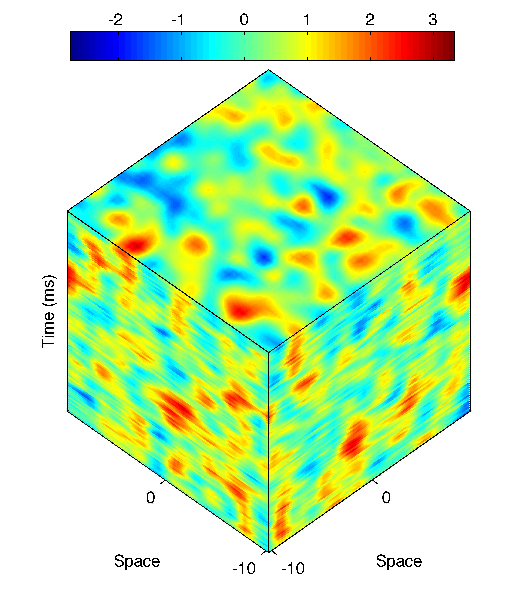
\includegraphics[scale=1]{./Graph/100FieldsColorbar.pdf}}
		\subfigure[]{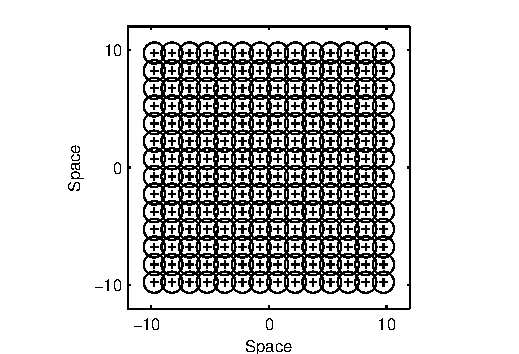
\includegraphics[scale=1]{./Graph/SensorArrangement.pdf}}
	\caption{The spatio-temporal dynamics of the field. (a) One example of 100 time instants of the simulated field using \eqref{eq:ConvolutionIntegral}-\eqref{eq:ObservationEquation}   with PBC. (b) Arrangement of the sensor kernels. 196 Gaussian sensor kernels are centered on the plus with the distance between adjacent sensors $2.5$ mm and the width $\sigma_m=0.9$ mm.}
	\label{fig:SimulatedData}
\end{figure}

The aim of this section is to demonstrate the performance of the proposed estimation scheme. Estimation results using two forms of the IDE are demonstrated. In each form of the IDE two different spatial mixing kernels, isotropic and anisotropic, were adopted. The first example uses a forward model in the form of the Amari style neural field model \cite{Amari1977} ($\xi\neq 0$). Sythetic data is generated using a nonlinear sigmoidal activation function and an activation function that has been linearized about the threshold. The second example uses a linear forward model that is consistent with the work of Dewar et al.~\cite{Dewar2007}, where the decay parameter $\xi=0$.

The actual spatial mixing kernels are defined as a sum of Gaussian basis functions in the form of
\begin{align}\label{eq:sumofGaussians}
 k\left(\mathbf{r}-\mathbf{r}'\right)=\sum_{i=0}^{n_{\theta}}\theta_i\psi_i\left(\mathbf{r}-\mathbf{r}'\right), 
 \end{align}
where $\theta_i$ is the weight and
\begin{equation}\label{eq:Kernelbasis}
	\psi_i=\exp{\left(-\frac{(\mathbf{r}-\mathbf{r}'-\boldsymbol\mu_i)^\top(\mathbf{r}-\mathbf{r}'-\boldsymbol\mu_i)}{\sigma_i^2}\right)}.
\end{equation}
The kernel parameters for each simulation are given in Table~\ref{table:KernelParameters}.
\begin{table}[htbp]
\begin{center}
{\tiny\begin{tabular}{lcccc} 
\hline\hline
\multicolumn{1}{c}{Parameter} & \multicolumn{ 2}{c}{Non-linear} & \multicolumn{ 2}{c}{linear}   \\  \cline{ 1- 5}   
\multicolumn{ 1}{c}{} & Iso & Aniso & Iso & Aniso \vspace{1 mm}\\ 
$\theta_i$ & $100, -80, 5$ & $80, -80, 5, 15$ &$100, -80, 5$&$200, -200$  \\ 
$\sigma_i$ & $1.8, 2.4, 6$ &$1.8, 2.4, 6, 2$ & $1.8, 2.4, 6$ & $2.4, 2.4$ \\ 
$\boldsymbol{\mu}_i$&$[0~0]^{\top}$& $3\times[0~0]^{\top}, [-3~0]^{\top}$ &$[0~0]^{\top}$  &$[-0.5~0]^{\top}$, $[0~0.5]^{\top}$  \vspace{2 mm}\\ \hline \hline
\end{tabular}}
\end{center}
\caption{Spatial mixing kernel parameters for different examples.}
\label{table:KernelParameters}
\end{table}
 In each example, data was generated using equation \eqref{eq:ConvolutionIntegral} and \eqref{eq:ObservationEquation} over the spatial region $\mathcal{S}=[-10,10]^2 $, assuming periodic boundary conditions (PBC), and sampled over $t=\left\lbrace1 \cdots 20000  \right\rbrace $ at 196 regularly spaced locations, with the sensor kernel defined by a Gaussian
\begin{equation}\label{eq:observationkernel}
 	m\left(\mathbf{r}-\mathbf{r}'\right) = \exp{\left(-\frac{(\mathbf{r}-\mathbf{r}')^\top(\mathbf{r}-\mathbf{r}')}{\sigma_m^2}\right)},
 \end{equation} 
 where $\sigma_m$ sets the observation kernel width and chosen to be $0.9$. The superscript $\top$ denotes the transpose operator. The observation noise variance $\sigma_{\varepsilon}^2$ is set to $0.1$. The field disturbance covariance function, $\gamma(\cdot)$ is modeled by a Gaussian with the width $\sigma_{\gamma}^2=1.3$ and $\sigma_d^2=0.1$. For estimation, the first 1000 samples discarded allowing the initial transients to die out.  The simulation parameters are summarized in Table~\ref{table:SimulationParameters}.
\begin {table}[t]
\begin{center}
	{\tiny\begin{tabular}{lllll}
	\hline \hline
	& Symbol & Quantity &Value& Units\\ 
	\hline 
	& Domain&&& \\
	& $\Delta$ &Spatial discretization step&0.5&mm \\ 
 	& $T_s$ &Time step&0.001&s \\ 
 	& $T$ &Number of time steps&20000&n.a. \\ 
 	&Model&&& \\
 	& $\varsigma$ &Sigmoidal's slope&0.56 \cite{Wendling2005}&mV$^{-1}$spike.s$^{-1}$ \\ 
 	& $z_0$ &Sigmoid's threshold &1.8 \cite{Marreiros2008}&mV \\ 
 	& $\xi$ &Decay parameter&0.9 &n.a. \\  
  & $\sigma_{\gamma}$ &Disturbance covariance width&1.3 &mm \\  
  & $\sigma_{d}$ &Disturbance variance&0.1 &mV \\  
  & $n_{y}$ &Number of sensors&196 &n.a. \\  
  & $\Delta_{y}$ &Distance between sensors&1.5 &mm \\  
  & $\sigma_{m}$ &Observation kernel width&0.9 &mm \\  
  & $\boldsymbol\Sigma_{\varepsilon}$ &Observation noise covariance&$0.1\times\mathbf{I}_{n_y}$ &mV$^2$ \\  
% 	&Spatial kernel&&& \\
%  	&Isotropic&&& \\
% & $\boldsymbol\theta$ &Connectivity kernel parameters&$[80~-80~5]^{\top}$& mVspike$^{-1}$ \\
% & $\boldsymbol\mu_i$ &Kernel centers&$[0~0]^{\top}$& mm \\  
% & $\sigma_{\psi_i}$ &kernel width parameters&$1.8, 2.4, 6$& mm \\  
%  	&Anisotropic&&& \\
% & $\boldsymbol\theta$ &Connectivity kernel parameters&$[80~-80~5~15]^{\top}$& mVspike$^{-1}$ \\
% & $\boldsymbol\mu_{1,2,3}, \boldsymbol\mu_4 $ &Vector of kernel centers&$[0~0]^{\top}, [-3~0]^{\top} $& mm \\    
% & $\sigma_{\psi_i}$  &Spatial kernel width parameters&$1.8, 2.4, 6, 2$& mm \\   
 	\hline \hline
	\end{tabular}}
 \caption {Parameters for the model. } 
 \label{table:SimulationParameters}
 \end{center}
 \end {table}
 One example of the simulated field over 100 time instants, showing stable dynamics along with the sensor arrangement are shown in \figurename{\ref{fig:SimulatedData}}.

In the first example, sigmoid's parameters, i.e slope and threshold, observation noise variance and time scale parameter are assumed to be known. In the second example observation noise variance is also unknown to the estimator. In this case the effect of the observation noise variance on the spatial mixing kernel estimate is also examined.
\subsection{Example I: Non-linear and linearized IDE model, $\xi\neq 0$}
In this example we consider Amari type neural field model and set the decay parameter, $\xi$  to 0.9 \cite{Freestone2011}. The parameters of the isotropic kernel are set to $\boldsymbol\theta=[100~-80~5]^{\top}$,  $\boldsymbol\mu_i=[0~0]^{\top}$, $\sigma_0=1.8$, $\sigma_1=2.4$ and $\sigma_2=6$, forming a semi-compact support Mexican-hat shape commonly used in the neural field modeling \cite{Amari1977,Atay2005,Breakspear2010}. For anisotropic kernel the weight vector is given by $\boldsymbol\theta=[80~-80~5~15]^{\top}$. The first three basis functions are located at $\boldsymbol\mu_{0,1,2}=[0~0]^{\top}$ and the forth one is located at $\boldsymbol\mu_3=[-3~0]^{\top}$. The widths of the basis functions are set to $\sigma_0=1.8$, $\sigma_1=2.4$, $\sigma_2=6$ and $\sigma_3=2$. Two sets of data were generated using the non-linear and linearized activation functions in the forward model where the estimations for the spatial mixing kernel and the disturbance covariance function were obtained using \eqref{eq:EM-Fourier_TF_of_Kernel} and \eqref{eq:EM-MMGFourier2} respectively. The results of the estimation along with true shape for isotropic and anisotropic spatial mixing kernels are shown in \figurename{\ref{fig:IsoNonlinear}} and \figurename{\ref{fig:AnisoNonlinear}} respectively, showing the ability of the proposed method to capture the spatial mixing kernel from observed field in both scenarios where data is generated either using non-linear or linearized activation functions.
\begin{figure*}[ht]
	\centering
		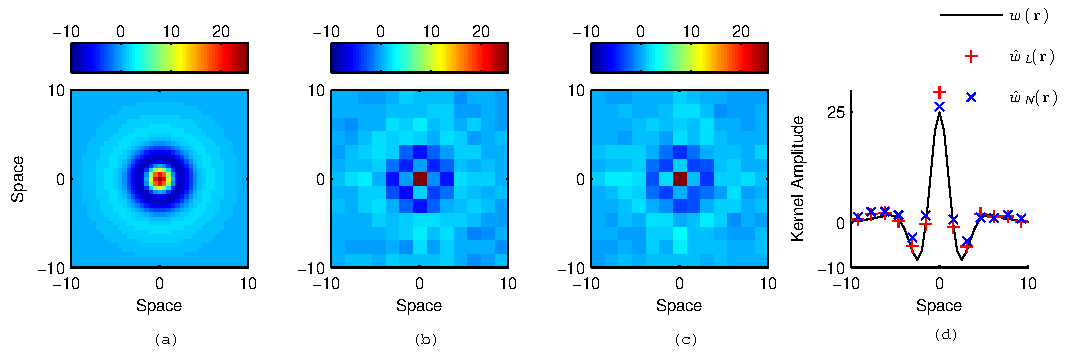
\includegraphics[scale=1]{./Graph/IsoKernelIEEE.pdf}
	\caption{Estimation of the isotropic kernel $\xi\neq 0$ using \eqref{eq:EM-Fourier_TF_of_Kernel}. High resolution actual spatial mixing kernel is shown in (a).   Estimated spatial mixing kernels at observation locations for non-linear and linearized forward model are shown in (b) and (c) respectively. Cross-sections of (a), (b) and (c) are shown in (d).}
	\label{fig:IsoNonlinear}
\end{figure*}
  
 \begin{figure*}[ht]
	\centering
		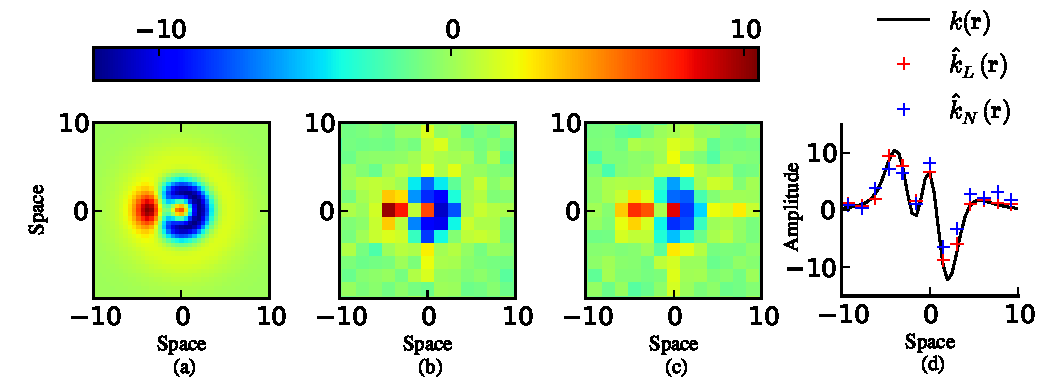
\includegraphics[scale=1]{./Graph/AnisoKernelIEEE1.pdf}
	\caption{Estimation of the anisotropic kernel $\xi\neq 0$ using \eqref{eq:EM-Fourier_TF_of_Kernel}. High resolution actual spatial mixing kernel is shown in (a).   Estimated spatial mixing kernels at observation locations for non-linear and linearized forward model are shown in (b) and (c) respectively. Cross-sections of (a), (b) and (c) are shown in (d).}
	\label{fig:AnisoNonlinear}
\end{figure*}

 Note the spatial mixing kernel can only be reconstructed at the observation locations which can be seen clearly in panel (d) of \figurename{\ref{fig:IsoNonlinear}} and \figurename{\ref{fig:AnisoNonlinear}}. Estimations of the disturbance covariance function are also depicted in \figurename{\ref{fig:DisturbanceNon}}, showing a small discrepancy at the origin. Note for the non-linear and linearized activation functions the results are very sensitive to observation noise, although a bound can be found for the observation noise, the exact value of this parameter is required in order to obtain fairly accurate estimations.
\begin{figure*}[ht]   
	\centering
		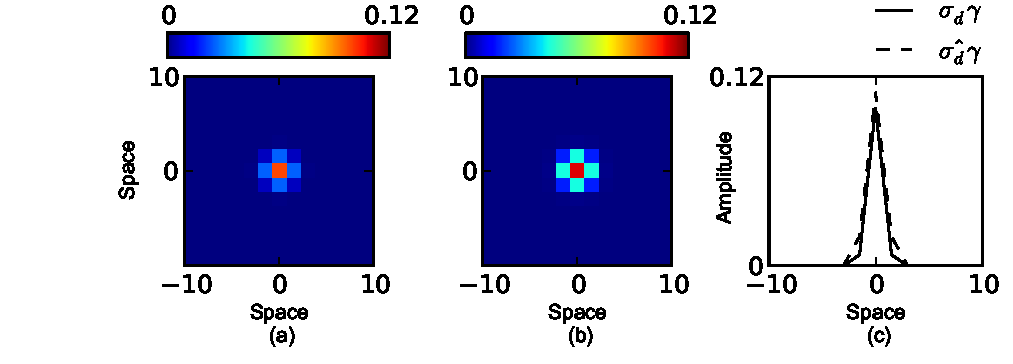
\includegraphics[scale=1]{./Graph/DisturbanceWidthEstimation.pdf}
	\caption{Estimation of the disturbance covariance function for anisotropic kernel where $\xi \neq 0$. Actual high resolution covariance function is shown in (a). Estimated covariance function using data obtained from non-linear and linearized forward model with their cross-sections at observation locations are shown in  (b), (c) and (d) respectively.}
	\label{fig:DisturbanceNon}
\end{figure*}


\subsection{Example II: Linear IDE model, $\xi=0$}
For this experiment the decay parameter, $\xi$ in \eqref{eq:ConvolutionIntegral} is set to zero describing a diffusive process described in \cite{Kot1992,Kot1996,Wikle1999,Xu2005}. The parameters of the isotropic kernel are the same as the previous example and the parameters of the anisotropic kernel are set to $\boldsymbol\theta=[200~-200]^{\top}$, $\boldsymbol\mu_0=[-0.5~0]^{\top}$, $\boldsymbol\mu_1=[0~0.5]^{\top}$, $\sigma_0=\sigma_1=2.4$.  
In this example solutions to the spatial mixing kernel and the disturbance covariance function are found by \eqref{eq:SimplifiedKernelSolution}   and \eqref{eq:DiffusionDisturbanceSolution} respectively. When this type of model is considered the solution to the kernel is not very sensitive to the observation noise variance, $\sigma_{\varepsilon}^2$ and any values close to the upper bound given by \eqref{eq:BoundOnObsVariance}, i.e., 
$0\le\sigma_{\varepsilon}^2\le 0.106$ yields reasonably accurate estimation. Using this upper bound the estimation of the kernel and the disturbance covariance functions are obtained (see \figurename{\ref{fig:DiffusionIso}} and \figurename{\ref{fig:DifussionAniso}). 
\begin{figure*}[h]
	\centering
		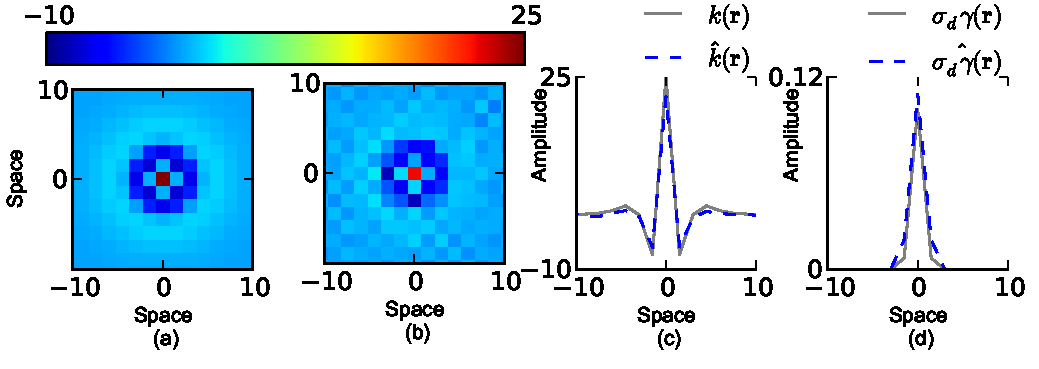
\includegraphics[scale=1]{./Graph/DisturbanceKernelEstimationLinearIso.pdf}
	\caption{Estimation of the isotropic kernel and disturbance covariance function for linear model using \eqref{eq:SimplifiedKernelSolution} and \eqref{eq:DiffusionDisturbanceSolution}. Actual and  estimated spatial mixing kernel at observation locations are shown in (a) and (b).  A cross-section of the actual kernel (solid line) and its estimate  (dashed line) are shown in (c). Cross-sections of the actual (solid line) and estimated (dashed line) disturbance covariance function are shown in (d).}
	\label{fig:DiffusionIso} 
	\end{figure*}
	
\begin{figure*}[h]
	\centering
		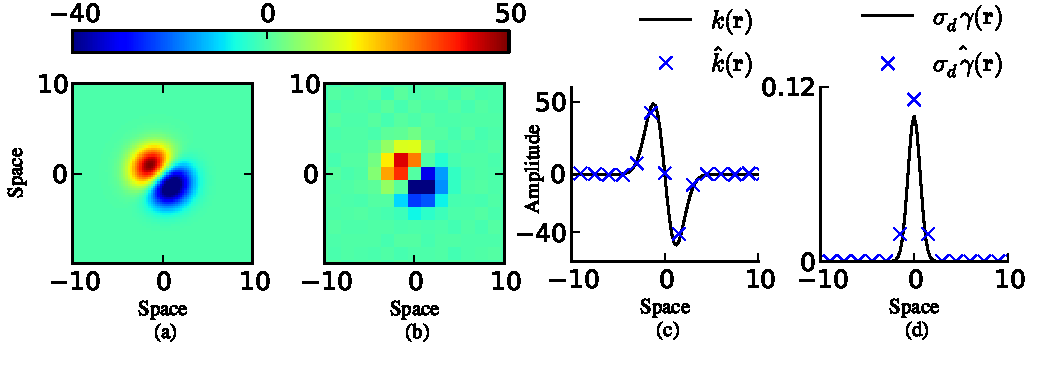
\includegraphics[scale=1]{./Graph/DisturbanceKernelEstimationLinearAniso.pdf}
	\caption{Estimation of the anisotropic kernel and disturbance covariance function for linear model using \eqref{eq:SimplifiedKernelSolution} and \eqref{eq:DiffusionDisturbanceSolution}. Actual and  estimated spatial mixing kernel at observation locations are shown in (a) and (b).  A cross-section of the actual kernel (solid line) and its estimate  (dashed line) are shown in (c). Cross-sections of the actual (solid line) and estimated (dashed line) disturbance covariance function are shown in (d).}
	\label{fig:DifussionAniso}
\end{figure*}  
The effect of $\sigma_{\varepsilon}^2$ on the kernel estimation is also shown in \figurename{\ref{fig:ObservationNoiseEffectonLinearIDE}}, showing distortion of the spatial mixing kernel where a value outside the bound is used.
\begin{figure*}[h]
	\centering
		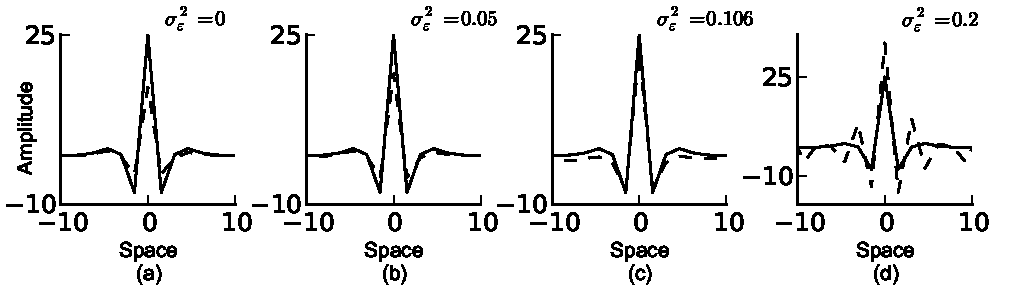
\includegraphics[scale=1]{./Graph/NoiseEffectIsoKernel.pdf}
	\caption{The effect of the observation noise on the spatial mixing kernel estimation for linear IDE model and $\xi=0$. Cross-sections of the estimated spatial mixing kernel for different values of the observation noise variance are shown. The minimum defined by inequality \eqref{eq:BoundOnObsVariance} is $0.106$. True and estimated kernel are shown by solid and dashed lines respectively.}
	\label{fig:ObservationNoiseEffectonLinearIDE}
\end{figure*}
\section{Conclusion}
\dean{a quick summary}

An efficient and novel approach to identifying spatio-temporal systems has been presented. The results demonstrated the ability to identify the spatial mixing kernel, disturbance and noise characteristics from noisy observations. This ability greatly facilitates the identification of the class of system which the IDE can represent.

\dean{what is different and where is it better}

\begin{enumerate}
	\item computational complexity
	\item implementation and algorithmic complexity
	\item can see how errors in other parameters might effect the kernel estimate
	\item an interesting aside is that it formally shows how synaptic time constants are linked to connectivity
	\item non prior knowledge of kernel shape is required and it may be isotropic
	\item can estimate disturbance and noise
\end{enumerate}


\dean{how this might compliment other schemes}

For more accurate estimation of the spatial kernel and also the inference of the underlying field the EM framework can be combined with the proposed method in this work. The estimated support of the kernel can be  used as a guide to constrain the placement of basis functions and the corresponding coefficients can be further corrected using the EM algorithm for more accurate representation of the mixing kernel structure. In fact, the correlation analysis can be considered a prerequisite for the EM algorithm described in \cite{Dewar2009}, where the approximated supports can be used to estimate the gain of the kernel and the field disturbance variance.                                             
         
The approximated support of the disturbance covariance function facilitates the application of the EM algorithm for estimating the temporal variance in the disturbance signal. This way the disturbance covariance matrix can be decomposed into two parts: an unknown scalar and a constant matrix depending only on the inferred spatial support. Therefore, the estimation problem of the disturbance covariance matrix breaks down to the estimation of a single scalar parameter, improving the accuracy and the convergence property of the algorithm.
                                                                                                                                                                     
\dean{alternatives to the IDECorr method}

An alternative to estimating the support of the kernel in a traditional state-space scheme is to place a regular grid of spatial mixing kernel basis functions over the entire spatial domain of the field. However, the estimate of the spatial extent of the mixing kernel greatly improves the speed of the estimation algorithm as the number of basis functions can be significantly reduced. This also improves the uncertainty in the estimated coefficients, as a lower number of unknown parameters needs to be estimated. 


\dean{extensions}

\begin{enumerate}
	\item second order 
 
\parham{ One extension to this framework is to include finite rise impulse response into the model, leading into a second-order IDE which can be written as two coupled first-order IDEs. This is particularly relevant if the proposed method is to be applied to electrophysiological data as the synaptic dynamics can be better approximated \cite{VanRotterdam1982}.}   
	\item automated placement of kernel basis functions
	\item freq analysis to define basis function width  
	\parham{One way to infer the spatial mixing kernel and the underlying field from observation is to find a finite dimensional state-space representation of the IDE using basis function decomposition. An approximation of the basis function widths can be determined using conventional spectral analysis of the observed field. However, it may be also possible to compute a closed-form solution of the basis functions ...  }
\end{enumerate}
In the case where the spatial process is observed at irregular locations, spatial interpolation maybe possible to apply in order to obtain a regular grid of observations to perform the proposed estimation framework.




% if have a single appendix:
 \appendix[Convolution and Correlation]
% or
% \appendices  % for no appendix heading
% do not use \section anymore after \appendix, only \section*
% is possibly needed
% use appendices with more than one appendix
% then use \section to start each appendix
% you must declare a \section before using any
% \subsection or using \label (\appendices by itself
% starts a section numbered zero.)
%  ###########################################
 \section{Convolution and Correlation}\label{ap:CorrelationAnalysis}
In this appendix the properties of the cross-correlation and the convolution used in Section~\ref{sec:EstimationMethod}   are derived. To show 
\begin{equation}\label{eq:app-ConvXcorRelation1}
 \left(a \ast b \right)\left(\boldsymbol\tau\right)  \star c\left(\boldsymbol\tau\right)  = a\left(-\boldsymbol\tau\right)\ast\left(b \star c\right)\left(\boldsymbol\tau\right)
\end{equation}
and
\begin{equation}\label{eq:app-ConvXcorRelation2}
(a \ast b)(\boldsymbol \tau) \star (a \ast b)(\boldsymbol\tau)=(a \star a)(\boldsymbol\tau)\ast(b \star b)(\boldsymbol\tau),
\end{equation}
first note that cross-correlation function is related to the convolution by \cite{Yarlagadda2009}
\begin{equation}\label{eq:app-ConvXcorRelation}
 \left(a \star b\right)\left(\boldsymbol\tau\right)= a\left(-\boldsymbol\tau\right)\ast b\left(\boldsymbol\tau\right).
\end{equation}
Therefore, \eqref{eq:app-ConvXcorRelation1} can be written as
\begin{align}
 \left(a \ast b\right)\left(\boldsymbol\tau\right) \star c\left(\boldsymbol\tau\right)&= \left(a \ast b\right)\left(-\boldsymbol\tau \right)\ast c\left(\boldsymbol\tau\right) \nonumber \\
&=a\left(-\boldsymbol\tau\right)\ast \left(b\left(-\boldsymbol\tau\right) \ast c\left(\boldsymbol\tau\right)\right)\nonumber \\
&=a\left(-\boldsymbol\tau\right)\ast\left(b\star c\right)\left(\boldsymbol\tau\right).
\end{align}
Similarly, \eqref{eq:app-ConvXcorRelation2} can be written as
\begin{align}
 (a \ast b)(\boldsymbol \tau) \star (a \ast b)(\boldsymbol\tau)&=(a \ast b)(-\boldsymbol\tau) \ast (a \ast b)(\boldsymbol\tau) \nonumber \\
&=a(-\boldsymbol\tau)\ast a(\boldsymbol\tau) \ast b(-\boldsymbol\tau)\ast b(\boldsymbol\tau) \nonumber \\
&=(a \star a)(\boldsymbol\tau)\ast(b \star b)(\boldsymbol\tau).
\end{align}     
%  \section{Linear IDE}\label{ap:linearIDE}  
% Consider the following homogeneous linear IDE
% \begin{equation}\label{app:DiscreteTimeModel}
% 	z_{t+1}\left(\mathbf{r}\right) = 
% 	\xi z_t\left(\mathbf{r}\right) + 
% 	T_s \int_\Omega { 
% 	    k\left(\mathbf{r}-\mathbf{r'}\right)z_t\left(\mathbf{r}'\right)
% 	\, \mathrm{d}\mathbf{r}'} 
% 	+ e_t\left(\mathbf{r}\right), 
% \end{equation}              
% then the results for the spatial mixing kernel and the covariance functions are simplified to
% \begin{equation}\label{app:EM-KernelSolution}
% 	k(\boldsymbol\tau) = \frac{1}{T_s }\mathcal{F}^{-1}\overline{\left\{\frac{\mathcal{F}\{\mathbf{E}[R_{y_{t+1}y_t}(\boldsymbol{\tau})]\}}{\mathcal{F}\{(\mathbf{E}\left[R_{y_ty_t}(\boldsymbol\tau)\right]\} - \sigma_{\varepsilon}^2 }-\xi\right\}}.
% \end{equation}  
% and
% \begin{align}\label{app:DiffusionDisturbanceSolution}
% 	&\gamma(\boldsymbol\tau) =\mathcal{F}^{-1}\left\lbrace \frac{1}{\tilde{m}(\boldsymbol\tau)}\Bigg[\left[\mathcal{F}\{\mathbf{E}[R_{y_{t+1}y_{t+1}}(\boldsymbol{\tau})]\}-\sigma_{\varepsilon}^2\right] \nonumber \right.\\
%  &\left. \left.- \left[\frac{\mathcal{F}\{\mathbf{E}[R_{y_{t+1}y_t}(\boldsymbol{\tau})]\}\mathcal{F}\left\{\mathbf{E}\left[R_{y_ty_{t+1}}(\boldsymbol\tau)\right] \right\}}{\mathcal{F}\{(\mathbf{E}\left[R_{y_ty_t}(\boldsymbol\tau)\right]\} - \sigma_{\varepsilon}^2}\right]\right]\right\rbrace.
% \end{align}                                                                                                                       
% This is in fact a spacial case for the general solutions given by \eqref{eq:Fourier_TF_of_Kernel} and \eqref{eq:EM-MMGFourier2} with $\varsigma=4$ and $z_0=0.5$. This can be further simplified by setting the decay parameter, $\xi=0$ to model diffusion processes.  In this case the solution for the kernel is given by
% \begin{equation}\label{app:DiffusionKernelSolution}
% 	k(\boldsymbol\tau) =\frac{1}{T_s }\mathcal{F}^{-1}\overline{\left\{\frac{\mathcal{F}\{\mathbf{E}[R_{y_{t+1}y_t}(\boldsymbol{\tau})]\}}{\mathcal{F}\{(\mathbf{E}\left[R_{y_ty_t}(\boldsymbol\tau)\right]\} - \sigma_{\varepsilon}^2 }\right\}}.
% \end{equation}                      
% Setting  the sampling time $T_s=1$ solves the linear IDE studied in \cite{Dewar2009, Scerri2009}. The disturbance covariance function solution remains unchanged, showing that the result is independent of the decay term. In this case the exact shape of the covariance function only depends on the observation noise variance and the observation kernel.            
%\appendices
%\section{Proof of the First Zonklar Equation}
%Appendix one text goes here.

% you can choose not to have a title for an appendix
% if you want by leaving the argument blank
%\section{}
%Appendix two text goes here.


% use section* for acknowledgement
%\section*{Acknowledgment}

% Can use something like this to put references on a page
% by themselves when using endfloat and the captionsoff option.
\ifCLASSOPTIONcaptionsoff
  \newpage
\fi



% trigger a \newpage just before the given reference
% number - used to balance the columns on the last page
% adjust value as needed - may need to be readjusted if
% the document is modified later
%\IEEEtriggeratref{8}
% The "triggered" command can be changed if desired:
%\IEEEtriggercmd{\enlargethispage{-5in}}

% references section

% can use a bibliography generated by BibTeX as a .bbl file
% BibTeX documentation can be easily obtained at:
% http://www.ctan.org/tex-archive/biblio/bibtex/contrib/doc/
% The IEEEtran BibTeX style support page is at:
% http://www.michaelshell.org/tex/ieeetran/bibtex/
 % \newpage
\bibliographystyle{IEEEtran}
% argument is your BibTeX string definitions and bibliography database(s)
\bibliography{IEEEabrv,IEEECorr}  
% <OR> manually copy in the resultant .bbl file
% set second argument of \begin to the number of references
% (used to reserve space for the reference number labels box)

% \begin{thebibliography}{1}
% 
% \bibitem{IEEEhowto:kopka}
% H.~Kopka and P.~W. Daly, \emph{A Guide to \LaTeX}, 3rd~ed.\hskip 1em plus
%   0.5em minus 0.4em\relax Harlow, England: Addison-Wesley, 1999.
% 
% \end{thebibliography}

% biography section
% 
% If you have an EPS/PDF photo (graphicx package needed) extra braces are
% needed around the contents of the optional argument to biography to prevent
% the LaTeX parser from getting confused when it sees the complicated
% \includegraphics command within an optional argument. (You could create
% your own custom macro containing the \includegraphics command to make things
% simpler here.)
%\begin{biography}[{\includegraphics[width=1in,height=1.25in,clip,keepaspectratio]{mshell}}]{Michael Shell}
% or if you just want to reserve a space for a photo:
% \begin{IEEEbiography}{Parham Aram}
% 
%  
% \end{IEEEbiography}
% 
% \begin{IEEEbiography}{Visakan Kadirkamanathan}
% % Biography text here.
% (M’90) received the
% B.A. and Ph.D. degrees in electrical and information
% engineering from the University of Cambridge, U.K.
% He held Research Associate positions at the University
% of Surrey, U.K., and the University of Cambridge,
% U.K., before joining the Department of Automatic
% Control and Systems Engineering, The University
% of Sheffield, U.K., as a Lecturer in 1993, where
% he is currently a Professor of Signal and Information
% Processing and is affiliated to the Centre for Signal
% Processing and Complex Systems. His research interests
% include nonlinear signal processing, system identification, intelligent control
% and fault diagnosis with applications in systems biology, aerospace systems,
% and wireless communication. He has coauthored a book on intelligent control
% and has published more than 120 papers in refereed journals and proceedings of
% international conferences.
% Prof. Kadirkamanathan is the Co-Editor of the International Journal of Systems
% Science and has served as an Associate Editor for the IEEE TRANSACTIONS
% ON NEURAL NETWORKS and the IEEE TRANSACTIONS ON SYSTEMS, MAN, AND
% CYBERNETICS, PART B.
%  \end{IEEEbiography}
% \begin{IEEEbiography}{Michael Dewar}
%  received the M.Eng. degree in
% control systems engineering and the Ph.D. degree
% in systems engineering both from The University of
% Sheffield, U.K., in 2002 and 2007, respectively.
%  He is currently working as
% a Research Associate in the Institute for Adaptive
% and Neural Computation, School of Informatics,
% The University of Edinburgh, U.K. 
% \end{IEEEbiography}

% if you will not have a photo at all:
% \begin{IEEEbiographynophoto}{John Doe}
% Biography text here.
% \end{IEEEbiographynophoto}

% insert where needed to balance the two columns on the last page with
% biographies
%\newpage

% \begin{IEEEbiographynophoto}{Jane Doe}
% Biography text here.
% \end{IEEEbiographynophoto}

% You can push biographies down or up by placing
% a \vfill before or after them. The appropriate
% use of \vfill depends on what kind of text is
% on the last page and whether or not the columns
% are being equalized.

%\vfill

% Can be used to pull up biographies so that the bottom of the last one
% is flush with the other column.
%\enlargethispage{-5in}



% that's all folks
\end{document}


